\documentclass{llncs}

\usepackage{proof}
\usepackage{mathpartir}
\usepackage{amsmath}
\usepackage{amssymb}
\usepackage{graphicx}

%\newtheorem{theorem}{Theorem}[section]
%\newtheorem{corollary}[theorem]{Corollary}
%\newtheorem{lemma}[theorem]{Lemma}
%\newtheorem{definition}[theorem]{Definition}

\def\qed{\unskip\kern 10pt{\unitlength1pt\linethickness{.4pt}\framebox(6,6){}}}

\newcommand{\fun}[1]{\mbox{\textbf{#1}}}
\newcommand{\lb}[1]{#1_{\downarrow}}
\newcommand{\ub}[1]{#1_{\uparrow}}
\newcommand{\varset}[1]{\mbox{$\cal{#1}$}}

\sloppy

\begin{document}

\title{Speed and Precision in Range Analysis}

\author{Victor Hugo Sperle Campos, Raphael Ernani Rodrigues, \\
Igor Rafael de Assis Costa and Fernando Magno Quint\~{a}o Pereira}

\institute{Department of Computer Science -- UFMG -- Brazil
\email{\{victorsc,raphael,igor,fernando\}@dcc.ufmg.br}
}


\maketitle

%mmmmmmmmmmmmmmmmmmmmmmmmmmmmmmmmmmmmmmmmmmmmmmmmmmmmmmmmmmmmmmmmmmmmmmmmmmmmmm
\begin{abstract}
Range analysis is a compiler technique that determines statically the lower and
upper values that each integer variable from a target program may assume
during this program's execution.
This type of inference is very important, because it enables several compiler
optimizations, such as dead and redundant code elimination, bitwidth aware
register allocation, and detection of program vulnerabilities.
In this paper we describe an inter-procedural, context-sensitive range analysis
algorithm that we have implemented in the LLVM compiler.
During the effort to produce an industrial-quality implementation of our
algorithm, we had to face a constant tension between precision and speed.
The foremost goal of this paper is to discuss the many engineering choices
that, due to this tension, have shaped our implementation.
Given the breath of our evaluation, we believe that this paper
contains the most comprehensive empirical study of a range analysis
algorithm ever presented in the compiler related literature.
\end{abstract}

%mmmmmmmmmmmmmmmmmmmmmmmmmmmmmmmmmmmmmmmmmmmmmmmmmmmmmmmmmmmmmmmmmmmmmmmmmmmmmm
\section{Introduction}
\label{sec:int}

% What range analysis is good for
Range analysis is a compiler technique whose objective is to determine
statically, for each program variable, limits for the minimum and maximum
values that this variable might assume during the program execution.
Range analysis is important because it enables many compiler optimizations.
Among these optimizations, the most well-known are dead and redundant
code elimination.
Examples of redundant code elimination include the removal of array bounds
checks~\cite{Bodik00,Logozzo08,Venet04} and overflow checks~\cite{Sol11}.
Additionally, range analysis is also used in bitwidth aware register
allocation~\cite{Barik06,Pereira08,Tallam03}, branch
prediction~\cite{Patterson95} and synthesis of hardware for specific
applications~\cite{Cong05,Lhairech10,Mahlke01,Stephenson00}.
Because of this importance, the programming language community has put much
effort in the design and implementation of efficient and precise range
analysis algorithms.

% The lack of a comprehensive empirical evaluation
However, the compiler related literature does not contain a comprehensive
evaluation of range analysis algorithms that scale up to entire programs.
Many works on this subject are limited to very small
programs~\cite{Mahlke01,Simon08,Stephenson00}, or, given their theoretic
perspective, have never been implemented in production
compilers~\cite{Gawlitza09,Lakhdar11,Su04,Su05}.
There are implementations of range analysis that deal with very large
programs~\cite{Bertrane10,Cousot09,Logozzo08,Oh11}; nevertheless, because
these papers focus on applications of range analysis,
and not on its implementation, they do not provide a thorough discussion
about their engineering decisions.
A noticeable exception is the recent work of Oh {\em et al.}~\cite{Oh12},
which discusses a range analysis algorithm developed for C programs that can
handle very large benchmarks.
Oh {\em et al.} present an evaluation of the speed and memory consumption of
their implementation.
In this paper we claim to push this discussion considerably further.

% Summary of our experiments
We have implemented an industrial-quality range analysis algorithm in the
LLVM compiler~\cite{Lattner04}.
While designing and implementing our algorithm we had to face several important
engineering choices.
Many approaches that we have used in an attempt to increase the precision of
our implementation would result in runtime slowdowns.
Although we cannot determine the optimum spot in this design space, given the
vast number of possibilities, we discuss our most important implementation
decisions in Section~\ref{sec:design}.
Section~\ref{sub:sccs} shows how we can improve runtime and precision
substantially by processing data-flow information in the strongly connected
components that underly our constraint system.
Section~\ref{sub:program_rep} discuss the importance of choosing a suitable
intermediate representation when implementing a sparse data-flow framework.
Section~\ref{sub:whole} compares the intra-procedural and the inter-procedural
versions of our algorithm.
The role of context sensitiveness is discussed in Section~\ref{sub:context}.
Finally, Section~\ref{sub:widen} discusses the different widening strategies
that we have experimented with.

% The history of our implementation
This work concludes a two years long effort to produce a solid and scalable
implementation of range analysis.
Our first endeavor to implement such an algorithm was based on Su and
Wagner's constraint system~\cite{Su04,Su05}.
However, although we could use their formulation to handle a subset of C-like
constructs, their description of how to deal with loops was
not very explicit.
Thus, in order to solve loops we adopted Gawlitza
{\em et al.}'s~\cite{Gawlitza09} approach.
This technique uses the Bellman-Ford algorithm to detect increasing or
decreasing cycles in the constraint system, and then saturates these cycles
via a simple widening operator.
A detailed description of our implementation has been published by
Couto and Pereira~\cite{Couto11}.
Nevertheless, the inability to handle comparisons between variables, and the
cubic complexity of the Bellman-Ford method eventually led us to seek
alternative solutions to range analysis.
This quest reached a pinnacle in the present work, which we summarize in this
paper.

\section{Brief Description of our Range Analysis Algorithm}
\label{sec:desc}

% Define the lattice, the constraints and the valuation I.
\noindent
\textbf{The Interval Lattice.}
Following Gawlitza {\em et al.}'s notation, we shall be performing arithmetic
operations over the lattice
$\cal{Z} = \mathbb{Z} \cup \{-\infty, +\infty\}$, where the ordering is
naturally given by $-\infty < \ldots -1 < 0 < 1 \ldots < +\infty$.
We let meet and join be the min and max operators respectively.
For any $x > -\infty$ we define:

\begin{tabular}{lcl}
$x + \infty = \infty$ & \mbox{\hspace{0.1cm}} & $x - \infty = - \infty$ \\
$x \times \infty = \infty$ if $x > 0$ & & $x \times \infty = -\infty$ if $x < 0$ \\
$0 \times \infty = 0$ & & $(-\infty) \times \infty = \ $ not defined $$ \\
\end{tabular}

From the lattice $\varset{Z}$ we define the product lattice
$\varset{Z}^2$, partially ordered by the subset relation $\sqsubseteq$, and
defined as $\varset{Z}^2 = \emptyset \cup \{[z_1, z_2] | \ z_1,z_2 \in \varset{Z}, \ z_1 \leq z_2, \  -\infty < z_2 \}$. The objective of range analysis is to determine a mapping
$I: V \mapsto \varset{Z}^2$ from the set of integer program variables
$V$ to intervals, such that, for any variable $v \in V$, if
$I(v) = [l, u]$, then, during the execution of the target program, any
value $i$ assigned to $v$ is such that $l \leq i \leq u$.

\noindent
\textbf{A Holistic View of our Range Analysis Algorithm.}
Figure~\ref{fig:algorithm} gives a global view of our range analysis
algorithm.
We perform range analysis in a number of steps, some of which are optional.
The optional parts improve the precision of the range analysis, at the expense of
a longer running time.
In Section~\ref{sec:design} we discuss in more detail these tradeoffs.

\begin{figure}[t!]
\begin{center}
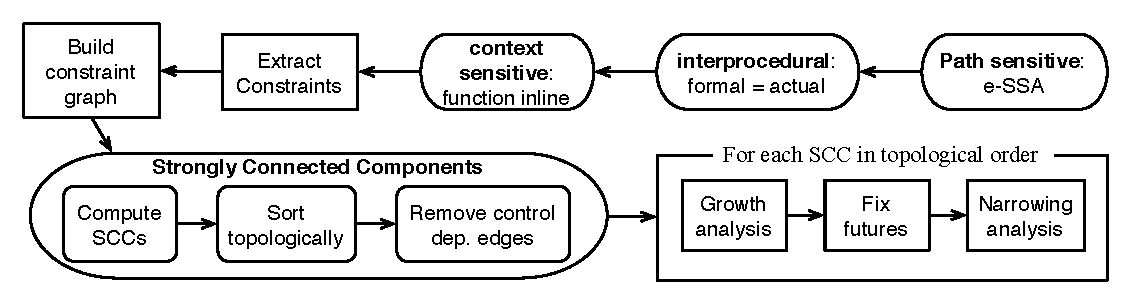
\includegraphics[width=\textwidth]{images/algorithm}
\end{center}
\caption{\label{fig:algorithm}
Our implementation of range analysis. Rounded boxes are optional modules.
The grey box is a module implemented in LLVM; the other parts are our
contributions.}
\end{figure}

We will illustrate the mandatory parts of the
algorithm via the example program in Figure~\ref{fig:overall_view}.
More details about each phase of the algorithm will be introduced in
Section~\ref{sec:design}, when we discuss our engineering decisions.
Figure~\ref{fig:overall_view}(a) shows an example program taken from the
partition function of the quicksort algorithm used by Bodik
{\em et al.}~\cite{Bodik00}.
Figure~\ref{fig:overall_view}(b) shows one possible way to represent this
program internally.
As we explain in Section~\ref{sub:program_rep}, a good program
representation helps range analysis to find more precise results.
In this example we chose a program representation called
Extended Static Single Assignment form~\cite{Bodik00}, which lets us solve range
analysis via a path sensitive algorithm.
This representation uses the $\phi$-functions typical in SSA form
programs~\cite{Cytron91}, plus {\em futures} (\textbf{ft}), which we shall
define later.
Figure~\ref{fig:overall_view}(c) shows the constraints that we extract from
the intermediate representation seen in part (b) of this figure.
From these constraints we build the {\em constraint graph} in
Figure~\ref{fig:overall_view}(d).
This graph is the main data-structure that we use to solve range analysis.
For each variable $v$ in the constraint system, the constraint graph has a node
$n_v$.
Similarly, for each constraint $v = f(\ldots, u, \ldots)$ in the constraint
system, the graph has an {\em operation node} $n_f$.
For each constraint $v = f(\ldots, u, \ldots)$ we add two edges to the
graph: $\overrightarrow{n_un_f}$ and $\overrightarrow{n_fn_v}$.
Some edges in the constraint graph are dashed.
These are called {\em control dependence edges}.
If a constraint $v = f(\ldots, \fun{ft}(u), \ldots)$ uses a {\em future}
bound from a variable $u$, then we add to the constraint graph a control
dependence edge $\overrightarrow{n_un_f}$.
The final solution to this instance of the range analysis problem is
given in Figure~\ref{fig:overall_view}(e).

\begin{figure}[t!]
\begin{center}
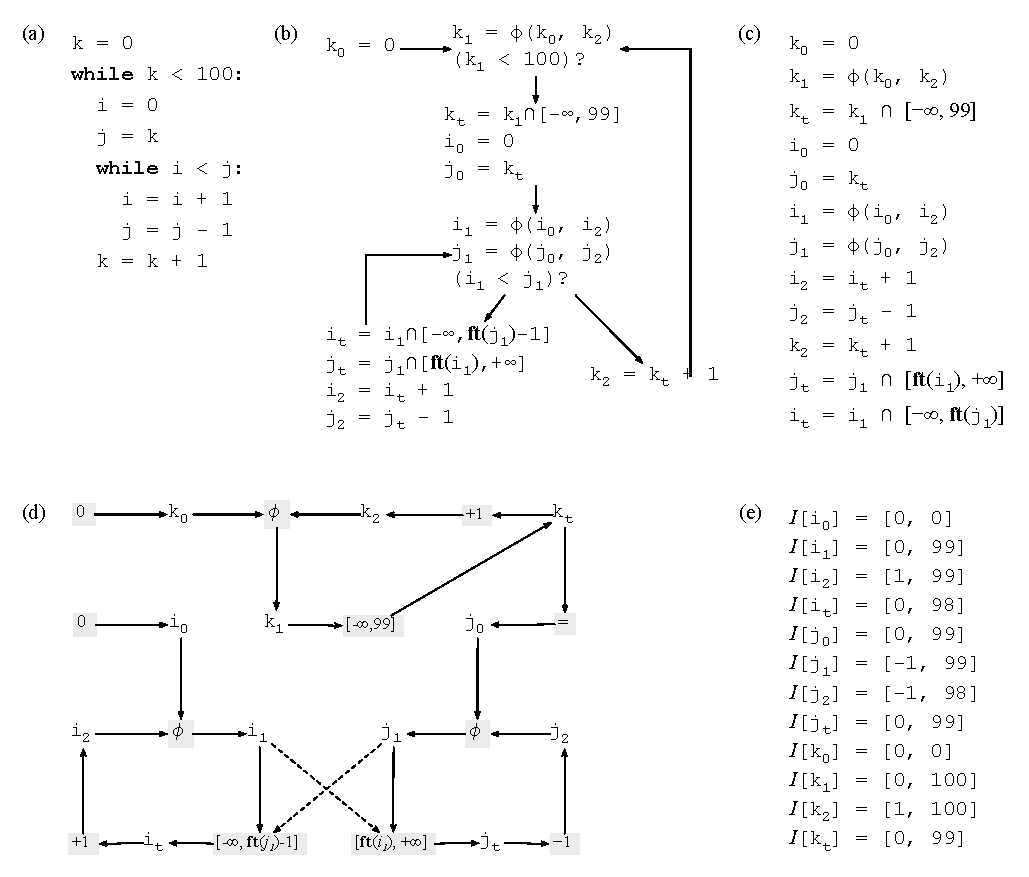
\includegraphics[width=\textwidth]{images/overall_view}
\end{center}
\caption{\label{fig:overall_view}
Range analysis by example.
(a) Input program.
(b) Internal compiler representation.
(c) Constraints of the range analysis problem.
(d) The constraint graph.
(e) The final solution.}
\end{figure}

\noindent
\textbf{The Micro Algorithm.}
We find the solution given in Figure~\ref{fig:overall_view}(e) in a
process that we call the micro algorithm.
This process is divided into three sub-steps:
(i) growth analysis;
(ii) future resolution and
(iii) narrowing analysis.

\noindent
\textbf{Growth analysis. }
The objective of growth analysis is to determine the growth behavior of
each program variable.
There are four possible behaviors:
(a) the variable is bound to a constant interval,
such as $k_0$ in Figure~\ref{fig:overall_view}(b).
(b) The variable is bound to a decreasing interval, i.e., an interval whose
lower bound decreases.
This is the case of $j_1$ in our example.
(c) The variable is bound to an increasing interval, i.e., its upper bound
increases.
This is the case of $i_1$ in the example.
(d) The variable is bound to an interval that expands in both directions.
The growth analysis uses an infinite lattice, i.e., $\varset{Z}^2$.
Thus, a careless implementation of an algorithm that infers growth patterns
might not terminate.
In order to ensure termination, we must rely on a technique called
{\em widening}, first introduced by Cousot and Cousot as a key component
of abstract interpretation~\cite{Cousot77}.
There are many different widening strategies.
We discuss some of them in Section~\ref{sub:widen}.

\noindent
\textbf{Future resolution. }
In order to learn information from comparisons between variables, such as
\texttt{i < j} in Figure~\ref{fig:overall_view}(a), we bind some intervals
to {\em futures}.
Futures are symbolic limits, which will be replaced by actual numbers once
we finish the growth analysis.
The ranges found by the growth analysis tells us which variables have fixed
bounds, independent on the intersections in the constraint system.
Thus, we can use actual limits to replace intersections bounded by futures.
Figure~\ref{fig:fix_intersects} shows the rules to perform these substitutions.
In order to correctly replace a future $\fun{ft}(v)$ that limits a variable
$v'$, we need to have already applied the growth analysis onto $v$.
Had we considered only data dependence edges, then it would be possible
that $v'$ be analyzed before $v$.
However, because of control dependence edges, this case cannot happen.
The control dependence edges ensure that any topological ordering of the
constraint graph either places $N_v$ before $N_{v'}$, or places these nodes
in the same strongly connected component.
For instance, in Figure~\ref{fig:overall_view}(d), variables $j_1$ and $i_t$
are in the same SCC only because of the control dependence edges.

\begin{figure}[t!]
\begin{center}
\begin{eqnarray*}
\begin{array}{c}
\inferrule{Y = X \sqcap [l, \fun{ft}(V) + c] \\ \ub{I(V)} = u}
{Y = X \sqcap [l, u + c]} \mbox{\hspace{0.3cm}} u, c \in \mathbb{Z} \cup \{-\infty, +\infty\}
\\
\\
\inferrule{Y = X \sqcap [\fun{ft}(V) + c, u] \\ \lb{I(V)} = l}
{Y = X \sqcap [l + c, u]} \mbox{\hspace{0.3cm}} l, c \in \mathbb{Z} \cup \{-\infty, +\infty\}
\end{array}
\end{eqnarray*}
\end{center}
\caption{\label{fig:fix_intersects}Rules to replace futures by actual
bounds. Given an interval $\iota = [l, u]$, we let $\lb{\iota} = l$, and
$\ub{\iota} = u$}
\end{figure}

\noindent
\textbf{Narrowing analysis.}
The growth analysis associates very conservative bounds to each variable.
Thus, the last step of our algorithm consists in narrowing these intervals.
We accomplish this step via Cousot and Cousot's classic narrowing
operator~\cite[p.248]{Cousot77}, which we show in
Figure~\ref{fig:crop_analysis}.

\begin{figure}[t!]
\begin{center}
\begin{eqnarray*}
\begin{array}{c@{\hspace{0.9cm}}c}
\inferrule{\lb{I(V)} = -\infty \\ \lb{e(V)} > -\infty}
{I(V) \leftarrow [\lb{e(V)}, \ub{I(V)}]}
&
\inferrule{\lb{I(V)} > \lb{e(V)}}
{I(V) \leftarrow [\lb{e(V)}, \ub{I(V)}]}
\\
\\
\inferrule{\ub{I(V)} = +\infty \\ \ub{e(V)} < +\infty}
{I(V) \leftarrow [\lb{I(V)}, \ub{e(V)}]}
&
\inferrule{\ub{I(V)} < \ub{e(V)}}
{I(V) \leftarrow [\lb{I(V)}, \ub{e(V)}]}
\end{array}
\end{eqnarray*}
\end{center}
\caption{\label{fig:crop_analysis}Cousot and Cousot's narrowing operator.
Function $e(V)$ is an abstract evaluation, on the interval lattice, of the
instruction that produces $V$.}
\end{figure}

\noindent
\textbf{Example.}
Continuing with our example, Figure~\ref{fig:ex_partition_grow_crop} shows
the application of our algorithm on the last strong component of
Figure~\ref{fig:overall_view}(d).
Upon meeting this SCC, we have already determined that the interval
$[0, 0]$ is bound to $i_0$ and that the interval $[100, 100]$ is bound to
$j_0$.
We are not guaranteed to find the least fixed point of a constraint system.
However, in this example we did it.
We emphasize that finding this tight solution was only possible because of
the topological ordering of the constraint graph in
Figure~\ref{fig:overall_view}(d).
Had we applied the widening operator onto the whole graph, then we would
have found out that variable $j_0$ is bound to $[-\infty, +\infty]$,
because
(i) it receives its interval directly from variable $k_t$, which is upper
bounded by $+\infty$, and
(ii) it is part of a negative cycle.
On the other hand, by only analyzing $j$'s SCC after we have
analyzed $k$'s, $k$ only contributes the constant range $[0, 99]$ to $j_0$.

\begin{figure}[t!]
\begin{center}
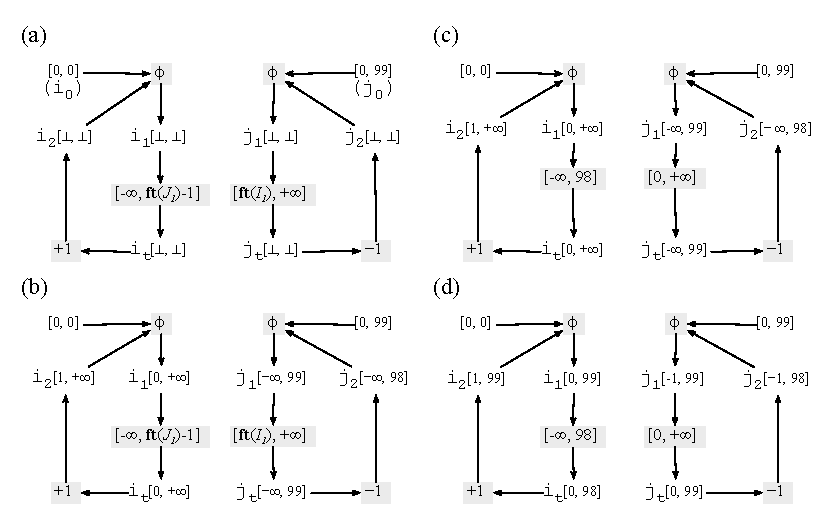
\includegraphics[width=\textwidth]{images/ex_partition_grow_crop}
\end{center}
\caption{\label{fig:ex_partition_grow_crop}
Four snapshots of the last SCC of Figure~\ref{fig:overall_view}(d).
(a) After removing control dependence edges.
(b) After running the growth analysis.
(c) After fixing the intersections bound to futures.
(d) After running the narrowing analysis.}
\end{figure}

%mmmmmmmmmmmmmmmmmmmmmmmmmmmmmmmmmmmmmmmmmmmmmmmmmmmmmmmmmmmmmmmmmmmmmmmmmmmmmm
\section{Design Space}
\label{sec:design}

As we see from a cursory glance at Figure~\ref{fig:algorithm}, our range
analysis algorithm has many optional modules.
These modules give the user the chance to choose between more precise results,
or a faster analysis.
Given the number of options, the design space of a range analysis algorithm
is vast.
In this section we try to cover some of the most important tradeoffs.
All the numbers that we show have been obtained as the average of 15 runs in
an Intel Core 2 Quad processor with 2.4 GHz, and 3.5 GB of main memory.
Figure~\ref{fig:space} plots, for the integer programs in the SPEC CPU 2006
benchmark suite, precision versus speed for different configurations of
our implementation.
Our initial goal when developing this analysis was to support a bitwidth-aware
register allocator.
Thus, we measure precision by the average number of bits that our
analysis allows us to save per program variable.
It is very important to notice that we do not consider constants in our statistics of precision.
In other words, we only measure bitwidth reduction in variables that a constant
propagation step could not remove.


\begin{figure}[t!]
\begin{center}
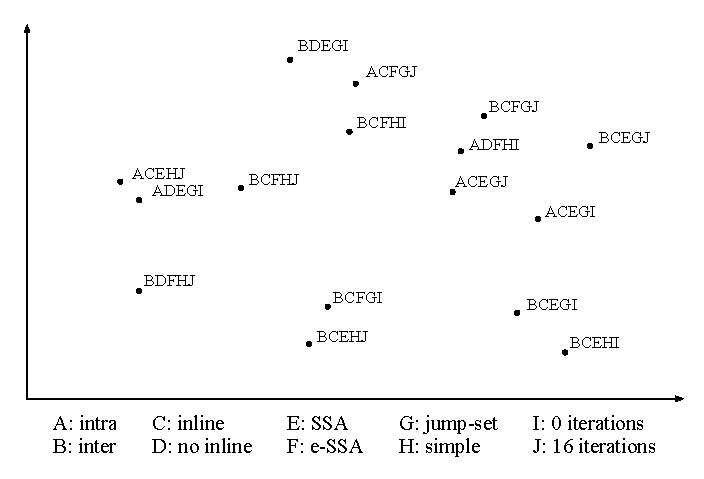
\includegraphics[width=\textwidth]{images/space}
\end{center}
\caption{\label{fig:space}
Design space exploration: precision (percentage of bitwidth reduction)
versus speed (secs) for different configurations of our algorithm analyzing
the SPEC CPU 2006 integer benchmarks.}
\end{figure}

\subsection{Strongly Connected Components}
\label{sub:sccs}

The greatest source of improvement in our implementation is the use of strongly
connected components.
To propagate ranges across the constraint graph, we fragment it
into strongly connected components, collapse each of these components into
single nodes, and sort the resulting directed acyclic graph topologically.
We then solve the range analysis problem for each component individually.
Once we have solved a component, we propagate its ranges to the next
components, and repeat the process until we walk over the entire constraint
graph.
It is well-known that this technique is essential to speedup constraint solving
algorithms~\cite[Sec 6.3]{Nielson99}.
In our case, the results are dramatic, mostly in terms of speed, but also in
terms of precision.
Figure~\ref{fig:impactSCC} shows the speedup that we gain by using strong
components.
We show results for the integer programs in the SPEC CPU 2006 benchmark suite.
In \texttt{xalancbmk}, the analysis on strong components is 450x faster.

\begin{figure}[t!]
\begin{center}
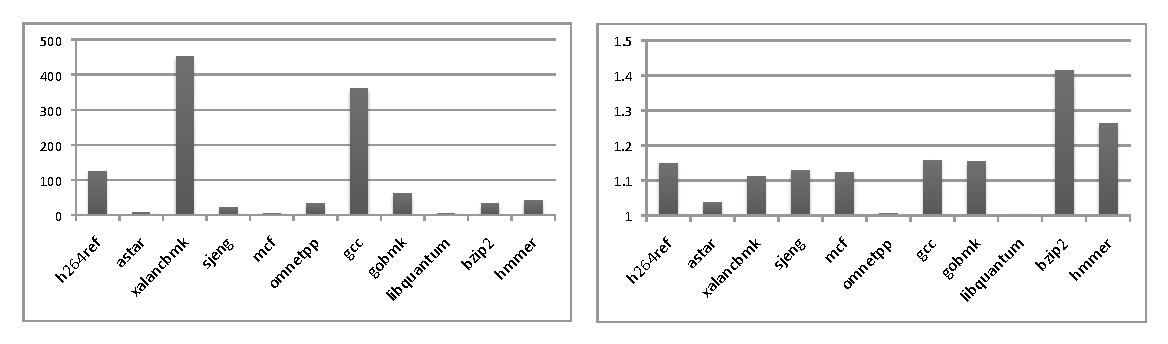
\includegraphics[width=\textwidth]{images/impactSCC}
\end{center}
\caption{\label{fig:impactSCC}
(Left) Bars give time to run our analysis without building strong components
divided by time to run the analysis on strongly connected components.
(Right) Bars give precision, in bitwidth reduction, that we obtain with strong
components, divided by the precision that we obtain without them.
}
\end{figure}

According to Figure~\ref{fig:impactSCC}, in some cases, as in \texttt{bzip2},
strong components increase our precision by 40\%.
The gains in precision happen because, by completely resolving a component,
we are able to propagate constant intervals to the next components, instead
of propagating intervals that can grow in both directions.
An an example, in Figure~\ref{fig:ex_partition_grow_crop} we pass the range
$[0, 99]$ from variable $k$ to the component that contains variable $j$.
Had we run the analysis in the entire constraint graph, by the time we
applied the growth analysis on $j$ we would still find $k$ bound to
$[0, +\infty]$.


\subsection{The choice of a program representation}
\label{sub:program_rep}

If strong components account for the largest gains in speed, the choice of
a suitable program representation is responsible for the largest gains in
precision.
However, here we no longer have a win-win condition: a more expressive
program representation decreases our speed, because it increases the
size of the target program.
We have tried our analysis in two different program representations: the
Static Single Assignment (SSA) form~\cite{Cytron91}, and the Extended Static
Single Assignment (e-SSA) form~\cite{Bodik00}.
The SSA form gives us a faster, albeit more imprecise, analysis.
Any program in e-SSA form has also the SSA core property: any variable name
has at most one definition site.
The contrary is not true: SSA form programs do not have the core e-SSA
property: any use site of a variable that appears in a conditional test
post-dominates its definition.
The program in Figure~\ref{fig:overall_view}(b) is in e-SSA form.
The live ranges of variables $i_1$ and $j_1$ have been split right after the
conditional test via the assertions that creates variables $i_t$ and $j_t$.
The e-SSA format serves well analyses that extract information from definition
sites and conditional tests, and propagate this information forwardly.
Examples include, in addition to range analysis, tainted flow
analysis~\cite{Rimsa11} and array bounds checks elimination~\cite{Bodik00}.

\begin{figure}[t!]
\begin{center}
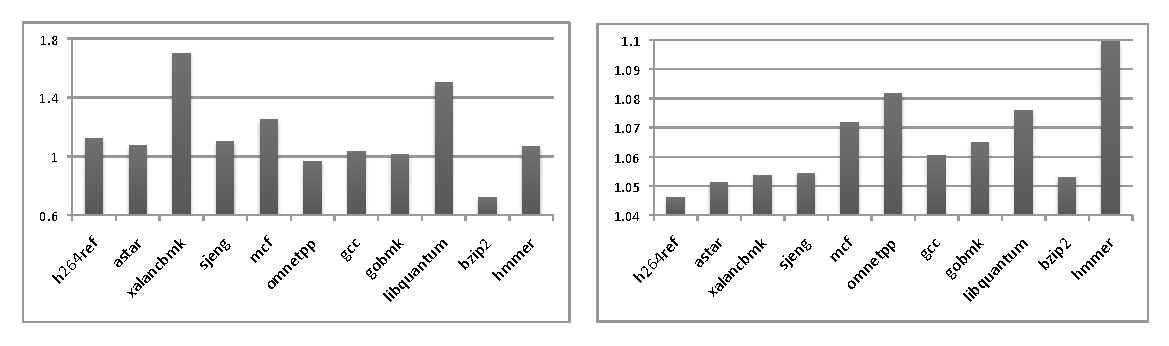
\includegraphics[width=1\textwidth]{images/impactESSA}
\end{center}
\caption{\label{fig:impactESSA}
(Left) Bars give the time to run analysis on e-SSA form programs divided by
the time to run analysis on SSA form programs.
(Right) Bars give the size of the e-SSA form program, in number of
assembly instructions, divided by the size of the SSA form program.}
\end{figure}

Figure~\ref{fig:impactESSA} compares these two program representations in
terms of runtime.
As we see in Figure~\ref{fig:impactESSA}(Left), the e-SSA form slows down our
analysis.
In some cases, as in \texttt{xalancbmk}, this slowdown increases execution
time by 71\%.
Runtime increases for two reasons.
Firstly, the e-SSA form programs are larger than the SSA form programs, as we
show in Figure~\ref{fig:impactESSA}(Right).
However, this growth is small: we did not verify any growth larger than 9\% in
any integer program of SPEC CPU 2006.
Second, the e-SSA form program has futures; hence requiring the future resolution
phase of our algorithm, which is not necessary in SSA form programs.
Nevertheless, whereas the e-SSA form slows down the analysis runtime, its gains in
precision are remarkable, as seen in Figure~\ref{fig:precESSA}.
These gains happen because the e-SSA format lets the analysis to use the
results of comparisons to narrow the ranges of variables.

\begin{figure}[t!]
\begin{center}
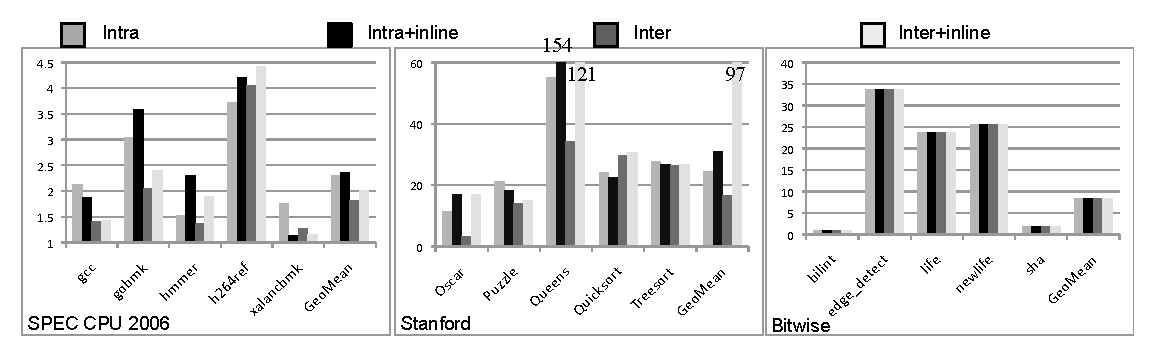
\includegraphics[width=1\textwidth]{images/precESSA}
\end{center}
\caption{\label{fig:precESSA}
The impact of the e-SSA transformation on precision for three different
benchmark suites. Bars give the ratio of precision (in bitwidth reduction),
obtained with e-SSA form conversion divided by precision without e-SSA form
conversion.}
\end{figure}

\subsection{Intra versus Inter-procedural Analysis}
\label{sub:whole}

A naive implementation of range analysis would be intra-procedural; that is,
would solve the range analysis problem once per each function.
However, we can gain in precision by performing it inter-procedurally.
An inter-procedural implementation allows the results found for a function $f$
to flow into other functions that $f$ calls.
Figure~\ref{fig:intra} illustrates the inter-procedural analysis for the
program seen in Figure~\ref{fig:overall_view}(a).
The trivial way to produce an inter-procedural implementation is to insert
into the constraint system assignments from the actual parameter names to the
formal parameter names.
In our example of Figure~\ref{fig:intra}, our constraint graph contains a flow
of information from $0$, the actual parameter, to $k_0$, the formal parameter
of function \texttt{foo}.

\begin{figure}[t!]
\begin{center}
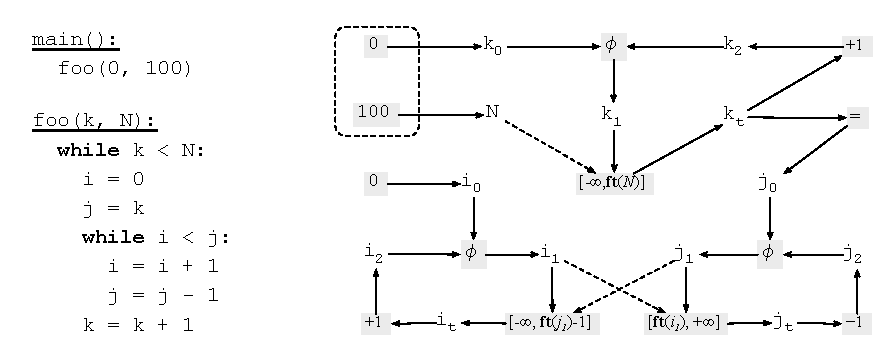
\includegraphics[width=\textwidth]{images/intra}
\end{center}
\caption{\label{fig:intra}
Example where an inter-procedural analysis is more precise than an
intra-procedural analysis.
}
\end{figure}

Figure~\ref{fig:wholeImpact} compares the precision of the intra and
inter-procedural analyses for the five largest programs in three different
categories of benchmarks: SPEC CPU 2006, the Stanford Suite~\footnote{\texttt{http://classes.engineering.wustl.edu/cse465/docs/BCCExamples/stanford.c}} and
Bitwise~\cite{Stephenson00}.
Our results for the SPEC programs were disappointing: on average, for
the five largest programs, the intra-procedural version of our analysis saves
5.23\% of bits per variable.
The inter-procedural version increases this number to 8.89\%.
A manual inspection of the SPEC programs reveals that this result is expected:
these programs use many external library functions, which we cannot analyze, and
their source codes do not provide enough explicit constants to power our analysis
up.
However, with numerical benchmarks we fare much better.
On average, our inter-procedural algorithm reduces the bitwidth of the
Stanford benchmarks by 36.24\%.
For Bitwise we obtain a bitwidth reduction of 12.27\%.
However, this average is lowered by two outliers: \texttt{edge\_detect} and
\texttt{sha}, which cannot be reduced.
The bitwise benchmarks were implemented by Stephenson
{\em et al.}~\cite{Stephenson00} to validate their bitwidth analysis.
Our results are on par with those found by the original authors.
The bitwise programs contain only the \texttt{main} function; thus, different
versions of our algorithm find the same results when applied onto these
programs.

\subsection{Context Sensitive versus Context Insensitive Analysis}
\label{sub:context}

Another way to increase the precision of range analysis is via a
context-sensitive implementation.
Context-sensitiveness allows us to distinguish different calling sites of
the same function.
Figure~\ref{fig:context} shows why the ability to make this distinction is
important for precision.
In Figure~\ref{fig:context}(a) we have two different calls of function
\texttt{foo}.
An usual way to perform a data-flow analysis inter-procedurally is to
create assignments between formal and actual parameters, as we show in
Figure~\ref{fig:context}(b).
If a function is called more than once, then its formal parameters will receive
information from many actual parameters.
We use the SSA's $\phi$-functions to bind this information together into a single
flow.
However, in this case the multiple assignment of values to parameters
makes the ranges of these parameters very large, whereas in reality they
are not.
As an example, in Figure~\ref{fig:context}(b), variable $k$ ends up
associated with the range $[0, 10^5]$, but in reality this variable contains
an interval that is only 100 units long.
A way to circumvent this source of imprecision is via function inlining,
as we show in Figure~\ref{fig:context}(c).
The results that we can derive for the transformed program are more
precise, as each input parameter is assigned a single value.

\begin{figure}[t!]
\begin{center}
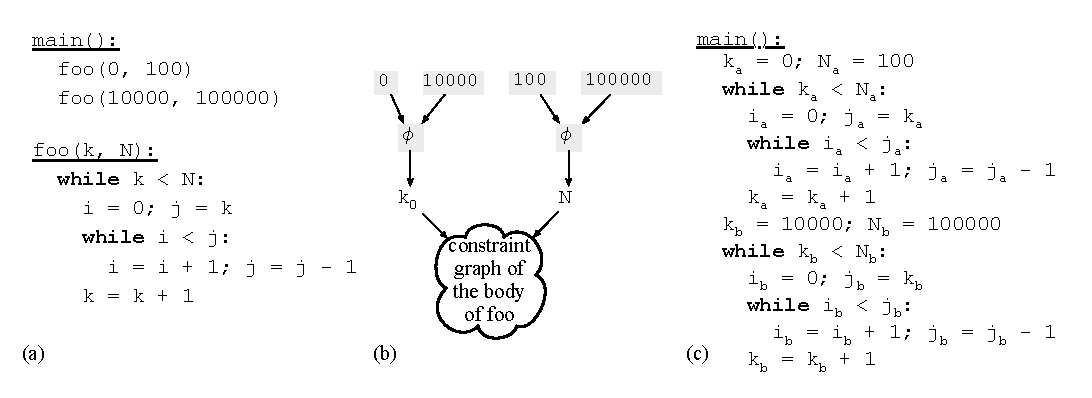
\includegraphics[width=\textwidth]{images/context}
\end{center}
\caption{\label{fig:context}
Example where a context-sensitive implementation improves the results of
range analysis.
}
\end{figure}

Figure~\ref{fig:wholeImpact} shows how function inlining modifies the
precision of our results.
It is difficult to find an adequate way to compare the precision of
our analysis with, and without inlining.
This difficulty stems from the fact that this transformation tends to change
the target program too much.
In absolute numbers, we always reduce the bitwidth of more variables after
function inlining.
However, proportionally function inlining leads to a smaller percentage of
bitwidth reduction for many benchmarks.
In the Stanford Collection, for instance, where most of the functions are
called in only one location, inlining leads to worse precision results.
On the other hand, for the SPEC programs, inlining, even in terms of
percentage of reduction, tends to increase our measure of precision.

\begin{figure}[t!]
\begin{center}
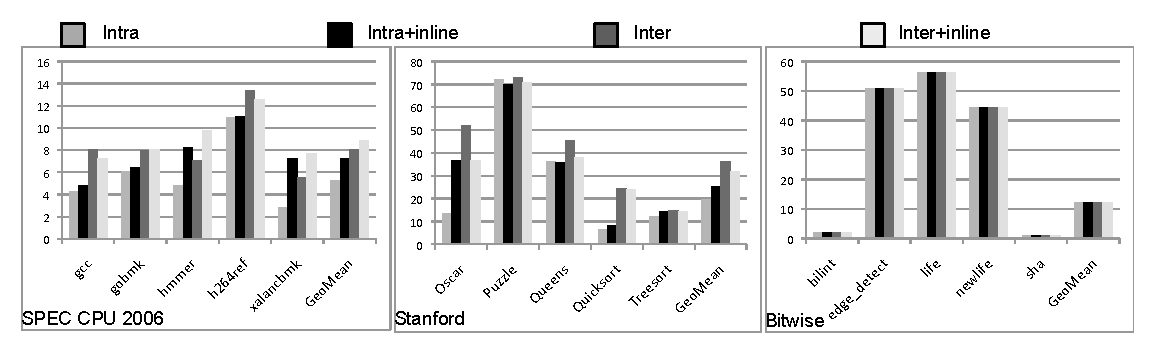
\includegraphics[width=\textwidth]{images/wholeImpact}
\end{center}
\caption{\label{fig:wholeImpact}
The impact of whole program analysis on precision. Each bar gives precision in
\%bitwidth reduction.}
\end{figure}

\noindent
\textbf{Intra vs Inter-procedural runtimes.}
Figure~\ref{fig:timeComp}(Right) compares three different execution modes.
Bars are normalized to the time to run the intra-procedural analysis
without inlining.
On average, the intra-procedural mode is 28.92\% faster than the inter-procedural
mode.
If we perform function inlining, then this difference is 45.87\%.
These numbers are close because our runtime is bound to the
size of the strong components.
We have observed that function inlining does not increase too much these
components.

\begin{figure}[t!]
\begin{center}
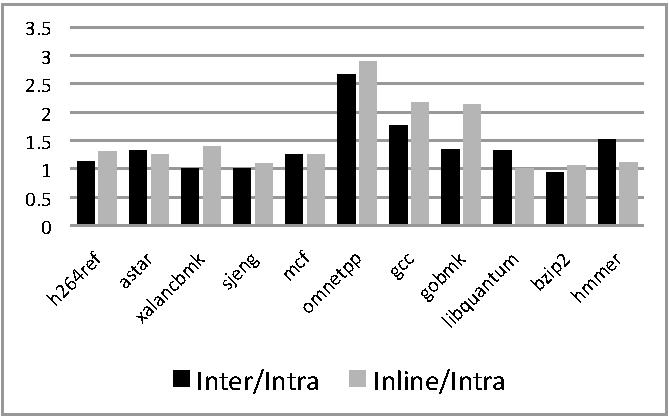
\includegraphics[width=0.45\textwidth]{images/timeIntraInterInline}
\end{center}
\caption{\label{fig:timeComp}
Runtime comparison between intra, inter and inter+inline versions of
our algorithm.
The bars are normalized to the time to run the intra-procedural analysis.
}
\end{figure}

\subsection{Choosing a Widening Strategy}
\label{sub:widen}

We have implemented the widening operator used in the growth analysis in
two different ways.
The first way, which we call {\em simple}, is based on Cousot and
Cousot's original widening operator~\cite{Cousot77}.
This operator is shown in Figure~\ref{fig:widening}, and it is the one
used in Figure~\ref{fig:ex_partition_grow_crop}(b).
The second widening strategy, which we call {\em jump-set widening} consists
in using the constants that appear in the program text, in sorted order, as
the next limits of each interval after widening is applied.
This operator is common in implementations of range
analysis~\cite[p.228]{Nielson99}.
There are situations in which jump-set widening produces better results
than the simple operator.
Figure~\ref{fig:jumpSet} shows an example taken from the code of
SPEC CPU \texttt{bzip2}.
Part of the constraint graph of the program in Figure~\ref{fig:jumpSet}(a)
is given in Figure~\ref{fig:jumpSet}(b).
The result of applying the simple operator is shown in
Figure~\ref{fig:jumpSet}(c).
Jump-set widening would use the lattice in Figure~\ref{fig:jumpSet}(d),
instead of the lattice in Figure~\ref{fig:widening}(Right).
This lattice yields the result given in Figure~\ref{fig:jumpSet}(e),
which is more precise.

\begin{figure}[t!]
\begin{center}
\begin{tabular}{c@{\hspace{1.5cm}}c}
\begin{minipage}{2cm}
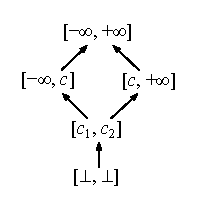
\includegraphics{images/growth_lattice}
\end{minipage}
&
\begin{minipage}{8cm}
\begin{small}
\begin{eqnarray*}
\begin{array}{c@{\hspace{0.5cm}}c}
\inferrule{I(V) = [\bot, \bot]}{I(V) \leftarrow e(V)}
&
\inferrule{\lb{e(V)} < \lb{I(V)} \\ \ub{e(V)} > \ub{I(V)}}
{I(V) \leftarrow [-\infty, +\infty ]}
\\
\\
\inferrule{\lb{e(V)} < \lb{I(V)}}
{I(V) \leftarrow [-\infty, \ub{I(V)}]}
&
\inferrule{\ub{e(V)} > \ub{I(V)}}
{I(V) \leftarrow [\lb{I(V)}, +\infty]}
\end{array}
\end{eqnarray*}
\end{small}
\end{minipage}
\end{tabular}
\end{center}
\caption{\label{fig:widening}
(Left) The lattice used in the simple widening strategy.
(Right) Cousot and Cousot's widening operator. We evaluate the rules from
left-to-right, top-to-bottom, and stop upon finding a pattern matching.}
\end{figure}


\begin{figure}[t!]
\begin{center}
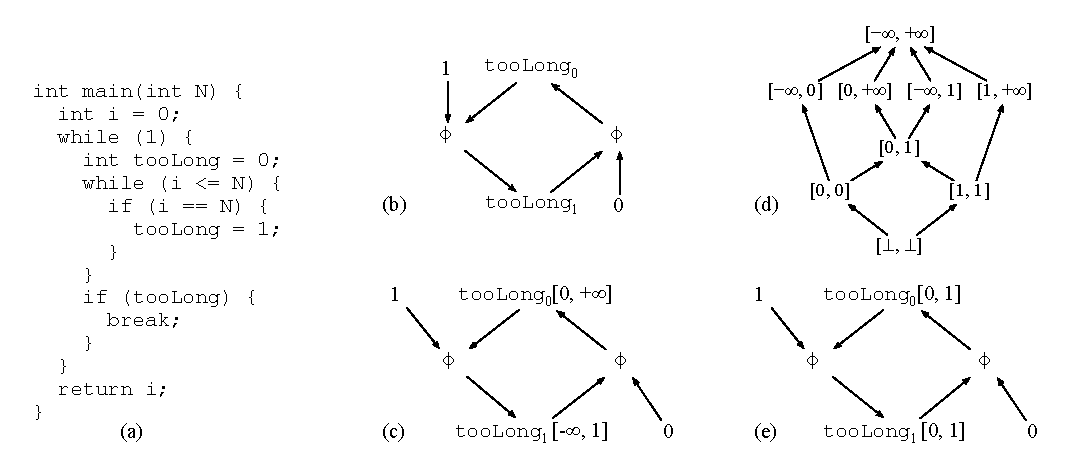
\includegraphics[width=1\textwidth]{images/jumpSet}
\end{center}
\caption{\label{fig:jumpSet}
An example where jump-set widening is more precise.}
\end{figure}

%%%%%%%%%%%%%%%%%%%%%%%%%%%%%%%%%%%%%%%%%%%%%%%%%%%%%%%%%%%%%%%%%%%%%%%%%%%%%%%%
Another way to improve the precision of growth analysis is to perform a few
rounds of abstract interpretation on the constraint graph, and to apply widening
only if this process does not reach a fixed point.
Each round of abstract interpretation consists in evaluating all the
constraints, and then updating the intervals that change from one evaluation to
the other.
For instance, in Figure~\ref{fig:jumpSet} one round of abstract interpretation,
coupled with the simple widening operator, would be enough to reach the
fixed point of that constraint system.
We have experimented with 0 and 16 iterations before doing widening, and the
overall result, for the programs in the SPEC CPU 2006 suite is given in
Figure~\ref{fig:space}.
Figure~\ref{fig:wideningPrec} shows some of these results in more detail
for the five largest benchmarks in this collection.
In general jump-set widening improves the precision of our results in
non-trivial ways.
Nevertheless, the simple widening operator preceded by 16 rounds of
abstract interpretation in general is more precise than jump-set widening
without any cycle of pre-evaluation, as we see in Figure~\ref{fig:wideningPrec}.

\begin{figure}[t!]
\begin{small}
\begin{center}
\renewcommand{\tabcolsep}{0.2cm}
\begin{tabular}{|c|c|c|c|c|c|c|c|c|c|c|c|c|} \hline
Benchmark &    Size & 0 + Simple &   16 + Simple &     0 + Jump & 16 + Jump \\ \hline
hmmer     &  38,409 &       9.98 & 11.40 (12.45) & 10.98 (9.11) & 11.40 (12.45) \\ \hline
gobmk     &  84,846 &       8.15 &  9.93 (17.92) &  9.02 (9.64) & 10.13 (19.54) \\ \hline
h264ref   &  97,494 &      12.58 &  13.11 (4.04) & 13.00 (3.23) & 13.11 (4.04) \\ \hline
xalancbmk & 352,423 &       7.71 &   7.98 (3.38) &  7.95 (3.02) & 7.98 (3.38) \\ \hline
gcc       & 449,442 &      16.09 &  16.63 (3.25) & 16.41 (1.95) & 16.64 (3.31) \\ \hline
\end{tabular}
\end{center}
\end{small}
\caption{\label{fig:wideningPrec}
Variation in the precision of our analysis given the widening strategy.
The size of each benchmark is given in number of variable nodes in the
constraint graph.
Precision is given in percentage of bitwidth reduction.
Numbers in parenthesis are percentage of gain over 0 + Simple.}
\end{figure}


%mmmmmmmmmmmmmmmmmmmmmmmmmmmmmmmmmmmmmmmmmmmmmmmmmmmmmmmmmmmmmmmmmmmmmmmmmmmmmm
\section{Final Remarks}
\label{sec:con}

This paper presents what we believe is the most comprehensive evaluation of
range analysis in the literature.
Altogether we have experimented with 32 different configurations of our
range analysis algorithm.
Our implementation is
publicly available at \texttt{http://code.google.com/p/range-analysis/}.
This repository contains instructions about how to deploy and use our
implementation.
We provide a gallery of examples, including source codes,
CFGs and constraint graphs that we produce for meaningful programs at
\texttt{http://code.google.com/p/range-analysis/wiki/gallery}.

\bibliographystyle{plain}
\bibliography{../references}

\end{document}
